\documentclass{tufte-handout}

%\geometry{showframe}% for debugging purposes -- displays the margins

\usepackage{amsmath}


% Set up the images/graphics package
\usepackage{graphicx}
\setkeys{Gin}{width=\linewidth,totalheight=\textheight,keepaspectratio}
\graphicspath{{graphics/}}


% The following package makes prettier tables.  We're all about the bling!
\usepackage{booktabs}

% The units package provides nice, non-stacked fractions and better spacing
% for units.
\usepackage{units}

% The fancyvrb package lets us customize the formatting of verbatim
% environments.  We use a slightly smaller font.
\usepackage{fancyvrb}
\fvset{fontsize=\normalsize}

% Small sections of multiple columns
\usepackage{multicol}

% Provides paragraphs of dummy text
\usepackage{lipsum}

% These commands are used to pretty-print LaTeX commands
\newcommand{\doccmd}[1]{\texttt{\textbackslash#1}}% command name -- adds backslash automatically
\newcommand{\docopt}[1]{\ensuremath{\langle}\textrm{\textit{#1}}\ensuremath{\rangle}}% optional command argument
\newcommand{\docarg}[1]{\textrm{\textit{#1}}}% (required) command argument
\newenvironment{docspec}{\begin{quote}\noindent}{\end{quote}}% command specification environment
\newcommand{\docenv}[1]{\textsf{#1}}% environment name
\newcommand{\docpkg}[1]{\texttt{#1}}% package name
\newcommand{\doccls}[1]{\texttt{#1}}% document class name
\newcommand{\docclsopt}[1]{\texttt{#1}}% document class option name


%%% Additions to template by DSL
\usepackage{hyperref} % provides \url{}
% remove separation between list items http://tex.stackexchange.com/a/10689/1783
\usepackage{enumitem}
\setlist{nosep}


\title{Shiitake Cultivation on (Small Logs, at Home)}
\author{David LeBauer}
\date{7 March 2015}  % if the \date{} command is left out, the current date will be used
\begin{document}

\maketitle% this prints the handout title, author, and date
\marginnote{\textsc{Contact:\\
David LeBauer\\
email: dlebauer@gmail.com
}}


\begin{abstract}
\noindent \textsc{Shiitake are delicious to eat and easy to grow.}
The objective of this two hour workshop is to introduce the basic steps required to grow shiitake on a log.
\sidenote{This is a truncated version of a one-day workshop that I orignially taught through the North Carolina Extension Service, and which I have more recently taught through the Land Connection here in Illinois. That class is aimed at commercial outdoor shiitake production on logs. Please contact me for details.}
Today's class will start with an overview of fungal ecology and physiology: the different types of fungi, how they grow, fruit, reproduce, and interact with one another and with plants.
This will provide a foundation for understanding how to cultivate and care for your logs and their fungal guests. Next, I will give an overview of the inoculation, care, and fruiting of shiitake on logs. The class will end with a hands-on section in which each student will be able to inoculate a log. 
Finally, we will discuss taking care of logs and how to encourage them to produce mushrooms. 
By the end of the class, students should be able to grow mushrooms on their own.
\end{abstract}


\marginnote{
\textsc{Agenda:}
\begin{description}
\item{3:10} Welcome \& Overview
\item Mushroom Ecology \& Physiology
\item Cultivating Growing Shiitake 
\item Hands-on inoculation
\item Clean up
\item Q\&A
\item{5:00} End
\end{description}
}


\section{Fungal Ecology \&  Physiology}



\subsection{The Carbon Cycle: Plants and Fungi}

\begin{marginfigure}
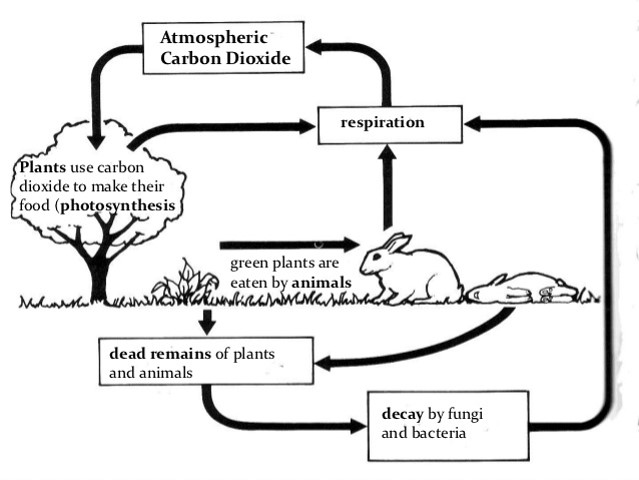
\includegraphics{figures/c-cycle.jpg}
\caption{Flows of carbon in an ecosystem.
Plants convert carbon dioxide in the atmosphere into biomass. Fungi, microbes, and animals convert plant material into soil organic matter, nutrients, and back to carbon dioxide.
Gardeners who focus on growing plants are missing out on half of this cycle.}
\end{marginfigure}

\newthought{Fungi play an important role} in the cycling of carbon and nutrient in ecosystems. Mushrooms are a type of fungi that produce a conspicuous 
fruiting body. Most mushrooms are either \emph{symbionts} or \emph{decomposers}.

Symbionts live in close relationships with plants. 
These organisms trade with plants - for example a fungus can mine nutrients in the soil more efficiently than a plant, and then exchange these nutrients with the plant for food.
These symbiotic mushrooms belong to a much larger group of fungi known as \emph{mycorrhizae}, and are associated with most plants. This group includes both \textsc{the most prized edible mushrooms} including porcini, chantrelles, and truffles as well as \textsc{the most deadly} such as the 'death cap'. 
Despite the ubiquity and deliciousness of these fungi, they are very difficult to cultivate, because both organisms must be cared for, the 'economic' conditions must be favorable for trade, and the environmental conditions must be favorable for fruiting.

\newthought{Shiitake, and most other cultivated mushrooms are decomposers}, unlike mycorrhizae, decomposers grow on dead plant material.  
There are many delicious edible mushrooms that have the simple habitat of growing on wood logs or chips, and the methods involved in their cultivation are relatively easy and rewarding. 
These include shiitake, oyster, white button, crimini, maitake / hen-of-the-woods, and many others.
Some decomposer fungi are also poisonous, but rarely deadly. 
Most edible decomposer mushrooms are easy to recognize with a little bit of experience, and there are no poisonous mushrooms that look anything like shiitake.

\subsection{The Fungal Life Cycle: Spores, Hyphae, and Mushrooms}

\begin{marginfigure}
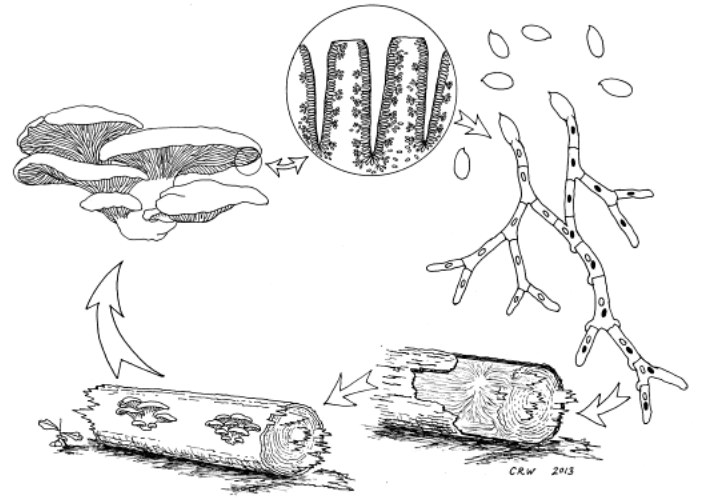
\includegraphics{figures/crw-mushroom-lifecycle}
\caption{The stages of a mushroom's life. "Farming the Woods"}
\end{marginfigure}

\newthought{Mushrooms are the reproductive structure produced by some fungi}. 
Fungi spend most of their lives as hyphae - a white mass tubular chain of cells that explore the soil, wood, or other substrate and release enzymes decomposing enzymes to convert it into food and air. 
Under the right conditions - for example when the fungus is running out of food or the weather becomes favorable for finding new substrate, the fungus will form a mushroom.
It is important to note that fungi have evolved to respond to specific environmental cues - the depletion of a food source coupled with particular changes in temperature and moisture availability. 
The mushroom raises into the air, and develops gills spores into the air so that once released, they will blow in the wind, and a few lucky ones will find a new home, and germinate.
Once the spores germinate, they begin to grow as hyphae, long thin chains of cells that explore and decompose wood, and find compatible hyphae to mate.

\subsection{Spawn}

\begin{marginfigure}
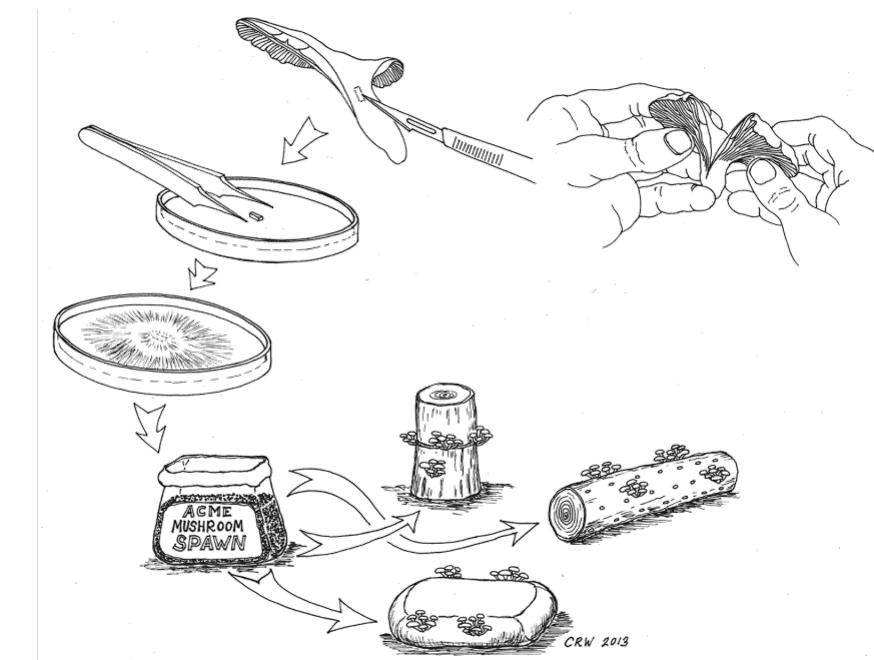
\includegraphics{figures/shiitake-spawn}
\caption{How mushroom spawn is made. First, tissue is removed from the mushroom fruitbody and transferred to  sterile culture. Then it is inoculated on a mixture of sawdust, wheat bran, and gypsum. Once the sawdust is colonized, it can be transferred to other logs. From "Farming The Woods" by Mudge and Gabriel.}
\end{marginfigure}

Spawn is a large mass of fungal hyphae grown on sawdust supplemented with a nitrogen source, commonly wheat bran. 
By growing on this sawdust, the fungus can increase its mass and growth rate. Once the sawdust is colonized, it is ready to transfer onto our logs.
The hyphae are transferred during this time of active growth  - if left too long, they will begin to loose their vigor and then fruit. 
Spawn should be purchased within a few weeks of inoculation, and kept in a cool, dark place or a refrigerator for longer periods. 

\newthought{There are Cold, Warm, and Wide climate range strains of Shiitake.}
Strains can be categorized as cold-weather (<50$^{\circ}$ F), midseason (50-64$^{\circ}$F), warm-weather (>68$^{\circ}$F), and wide range strains (41-95$^{\circ}$F). 
Growing a mixture of strains can extend the growing season. 
Warm weather strains grow more quickly, while cold weather strains produce fewer but higher quality mushrooms and will continue to produce for more seasons than faster growing strains because by growing more slowly, they conserve their food resources.

Strains vary in moisture requirement, preferred wood species, mushroom size and quality, colonization rate, and climate adaptation. 
Starting with a mixture of strains not only extends the season,  but also allows the grower to identify which ones are most
suitable to the climate of your log yard as well as your management
and marketing strategy.

\section{From Trees to Logs}

\begin{marginfigure}
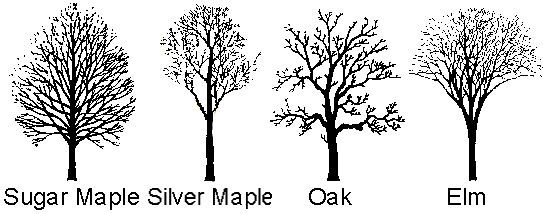
\includegraphics{figures/tree-forms}
\caption{Many trees have distinctive overall shapes; the scraggly nature of this oak is typicall \href{http://www.lostrivers.ca/content/points/treeswinter.html}{lostrivers.ca}}
\end{marginfigure}

\newthought{It is best to manually harvest fresh logs from healthy trees}\sidenote{The landscape recycling center on University Ave in Urbana is an excellent local source of fresh-cut logs.}. 
Machine harvested logs (as found in lumberyards) often these have bark damaged that will make logs susceptible to drying and infection. 
Logs with discoloration of the wood seen on the ends have been colonized by other fungi and should not be used because the shiitake will be fighting an uphill battle as the late comer to the competition for room on the log.
Hopefully this makes it clear that firewood is not suitable for shiitake production - it is old, dry, split, and likely already colonized.

\begin{marginfigure}
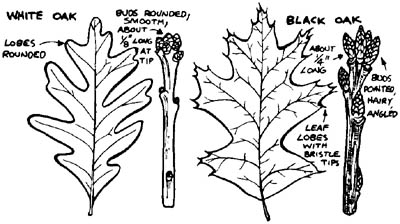
\includegraphics{figures/oak-leaves-twigs}
\caption{The leaves of common midwest oaks are lobed; all oaks have buds clustered at the end of the twig, and have opposite branching (unlike maple and ash)  
\href{http://www.michigan.gov/dnr/0,4570,7-153-10370_12148-61306--,00.html}{Fom "Forest Foods Deer Eat", Michigan Department of Natural Resources}
}
\end{marginfigure}

\subsection{Selecting Trees}


\newthought{Oaks are recommended} when available; indeed Shiitake means "oak mushroom" in Japanese.   
Oaks are easy to recognize, even in the winter, because of the overall form, the clustered buds, alternating branches, and the presence of oak leaves on the ground.  

Other excellent trees suitable for growing Shiitake include Maple, Ironwood, Cherry, and Sweetgum.
There are many species to avoid, including Aspen, Willow, Hickory, Ash, Elm, Locust, and conifers such as fir, pine, or spruce\sidenote{See also species chart from Field and Forest \href{http://www.fieldforest.net/pdfs/Tree Species Chart.pdf}{www.fieldforest.net}}.

\section{Inoculating Logs}

\marginnote{
\textsc{Materials}
\begin{description}
\item sturdy table
\item 12mm drill bits with collar 
\item spawn plunger
\item high speed drill 
\item wax (cheese or bees)
\item propane torch, stove, or hot plate
\item aluminum labels and nails
\end{description}
}


\subsection{The Inoculation Workflow}

An inoculation table will get covered in wax, and should allow logs to easily roll or slide down the assembly line. 
A metal cattle gates propped up on two
sawhorses work very well because they
facilitate rolling logs down the line while
allowing sawdust, spawn, and wax to drip
through. 
Labels made of small aluminum tags that can be hammered into the ends of logs are available from most mushroom supply companies (see "Sources" below), and should be marked with the strain used and date inoculated.


\begin{figure}
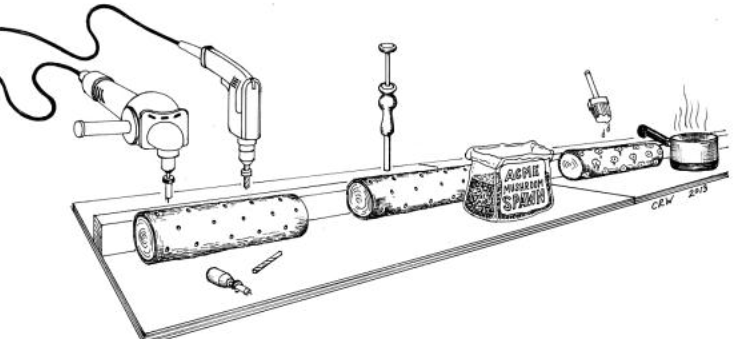
\includegraphics{figures/innoculation-workflow}
\caption{Overview of steps required to inoculate logs: drilling, inoculating, and waxing. (From "Farming the Woods")}
\end{figure}

If available, there should be one driller, two inoculators, and one waxer.
The second inoculator can also handle miscellaneous tasks such as refilling spawn and wax.
Spawn can be placed into an old coffee can. 
Drill holes every 6" in a line down the length of the log, rotate so the next line will be 3" below, and stagger the holes to form a diamond pattern. 
A self-taping drill bit is faster because it pulls the drill into the log.
Keep the drill running the entire time it is in the hole so that it will easily come out of the wood. 
The spacing of holes is just a guide to maximize colonization rate
and minimize damage to the bark. 
Roll the log to the inoculators, who then use plungers to fill holes with spawn.
Next, the holes are waxed to prevent
drying and infection. 
Wax should be melted in a tin can, and a paintbrush or similar device is used to cover each hole with wax.
Add a label with the date of inoculatoin and strain, as this will help you to assess
when and how much shiitake are produced
by each strain.

\section{Spawn Run}

\newthought{The spawn run is the time when the shiitake mycelium colonizes the log.} This should take about six months for our logs, though can take up to two years depending on strain, temperature, log size, and wood species.
This is the time when the logs are most sensitive to contamination and dessication, either of which could compromise the success of your log.
\emph{Shiitake will not survive if the logs get to dry}.

\newthought{It is important to maintain sufficient moisture in the log.} 
The easiest way to do this is to soak the log overnight every 4 weeks in non-chlorinated water\sidenote{Let tap water sit 24 hours to evaporate chlorine}. 
This can be done in a sink or bathtub.
When the log is young, it will float - place a weight on top to keep it submerged.


\newthought{Shiitake need fresh air and light to grow}.

After the spawn run, the logs are less susceptible to contamination because most of the wood substrate has been colonized by shiitake.
Inoculated logs may be placed either inside or outside.
If outside, the log should not be in the direct sun, not under a roof, and not in contact with the soil.
The ideal place for these logs is in the shade, preferably under an evergreen tree that provides shade throughout the winter and inhibits the growth of competitor fungi.
You can also cover the logs with shade cloth or pine branches to slow evaporation.
If growing indoors, keeping the log loosely covered with plastic can help to retain moisture, but it needs some light as well as some air flow - both for the oxygen as well as to prevent it from being too wet.

During dry summers, it may be necessary to water logs every week or two; it is preferable to water thoroughly but infrequently to allow the inside to get moist and the bark to dry out and remain dry. 

Colonization can be observed as creamy whitish discoloration at the ends of the log (under the wax) or seen by cutting through the bark with a knife.

\section{Fruiting}

Fruiting requires proper temperatures and moisture, and this depends on the strain.
To force-fruit an indoor log, either a) add ice to the 24 hour soaking tank or b) put the log in the refrigerator overnight following the soaking.
After fruiting, logs should be given eight to twelve weeks to recover before the next fruiting. 

\begin{marginfigure}
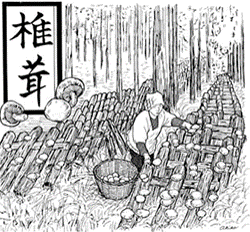
\includegraphics{figures/shiitake-harvest}
\caption{Harvesting shiitake from logs. Mitoku Products, www.mitoku.com}
\end{marginfigure}

Within a week or two of soaking, mushrooms will begin to fruit and pinheads - small primordial mushrooms - will begin to form. These are baby mushrooms and at this stage they are susceptible to freezing (if outside) or drying, which would prevent them from maturing into an edible mushroom. 
If the air is dry, lightly mist the logs and wet the surrounding ground to increase humidity.
For an indoor log, a transparent plastic bag can be placed over the log to help conserve moisture until the pins have matured, but care should be taken to prevent the bag from touching too much of the log.

Depending on temperature and strain, it may take one to three weeks from initiation to harvest. 
As the mushroom matures, a heavy rain can ruin a crop by making it soggy and unpalatable. 
For this reason, it is wise to cover fruiting logs that are outside. 

\begin{marginfigure}
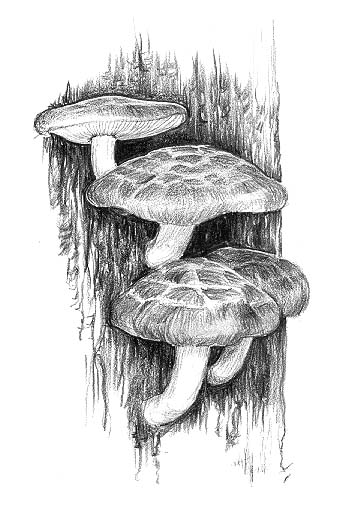
\includegraphics{figures/shiitake}
\caption{Shiitake mushrooms ready for harvest. www.mykoweb.com}
\end{marginfigure}

\section{References}

%\marginnote{

\subsection{Further Reading}
\begin{description}
\item \emph{How to Care for and Fruit Your Shiitake Mushroom Log}. Doug and Sondra Williams, Lost Creek Mushroom Farm \href{http://shiitakemushroomlog.com/care&handling.html}{shiitakemushroomlog.com}
\item[Farming the Woods:] An Integrated Permaculture Approach to Growing Food and Medicinals in Temperate Forests. Mudget and Gabriel 2014.  Chelsea Green Publishing. 359p.
\item[Mycelium Running:] How Mushrooms Can Help Save the World Stamets 2011. Ten Speed Press 435p
\end{description}

\subsection{Sources of Spawn and Supplies}

\begin{description}
\item[The Mushroom People] The Farm, TN. %Spawn and supplies for growing a variety of mushrooms. 
www.mushroompeople.com
\item[Field and Forest Products] Mary Ellen Kozak \& Joseph Krawczyk 
%have been growing shiitake and supplying farmers with spawn for over 30 years and are very helpful in solving problems. 
www.fieldforest.net
\item[Fungi Perfecti] Paul Stamets 
%of Ted "How Mushrooms can Save the World" fame, also author of canonical books, including "The Mushroom Cultivator" and "Growing Gourmet and Medicinal Mushrooms", and "Mycelium Running". 
www.fungi.com
\end{description}

%}%end marginnote

\end{document}